\chapter{Результаты} 
\label{chapter3}

\todo{интерпретация результата?}

\todo{REWRITE}

Зафиксируем следующую геометрию волновода:
\begin{ilist}
# $L_x = 200$ боровских радиусов (порядка 10 нм);
# $L_y = 100$ боровских радиусов (порядка 5 нм);
# $H = 100$ боровских радиусов (порядка 5 нм);
# $S = 10$ боровских радиусов (порядка 0.5 нм).
\end{ilist}
Пусть слева поступает входящая волна на первой моде:
\[
\psi_{inc}(x, y) = \sqrt{\frac{2}{H}} \sin(\frac{\pi}{H} y) e^{i \sqrt{E - \pi^2 / H^2}}
\]
Далее приведены результаты, полученные в рамках подхода, описанного в главе 2.
\section{Зависимость коэффициента прохождения от энергии входящей волны при фиксированной геометрии резонатора}
% \begin{figure}[H]
% 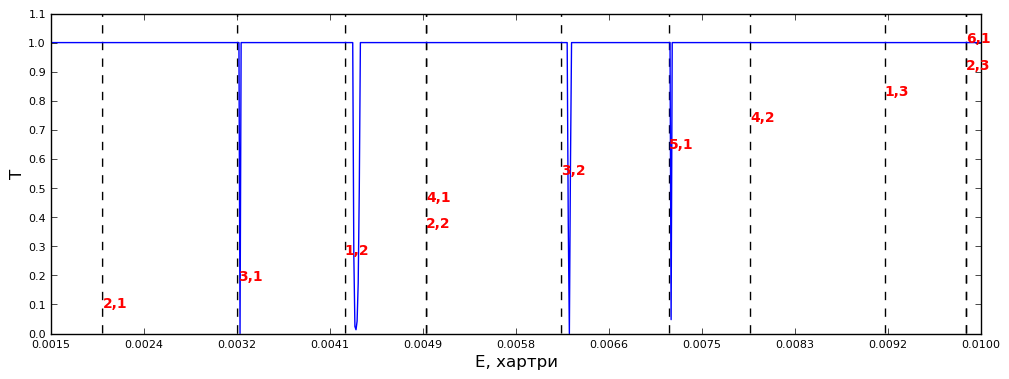
\includegraphics[width=1.0\textwidth]{transmission_all.png}
% \caption{Зависимость коэффициента прохождения от энергии при фиксированной геометрии. Вертикальные пунктирные линии соответствуют собственным энергиям резонатора, красными парами чисел обозначены номера состояний.}
% \label{fig:transmission_all}
% \end{figure}
% Как и ожидалось, в большинстве случаев коэффициент прохождения равен $1$. Падения коэффициента прохождения соответствуют тому, что волновая функция «чувствует» резонатор при некоторых энергиях, имеющих некоторую связь с собственными энергиями резонатора.

\section{Плотности вероятности}
% \begin{figure}[H]
% 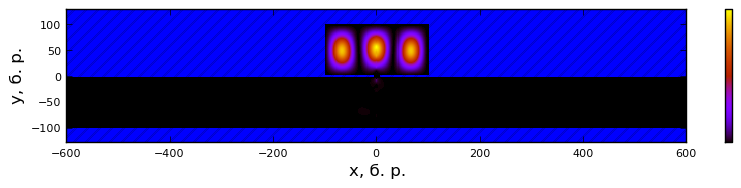
\includegraphics[width=1.0\textwidth]{pdensity_31_r.png}
% \caption{Плотность вероятности в резонансной точке.}
% \label{fig:pdensity_31_r}
% \end{figure}
% На рисунке~\ref{fig:pdensity_31_r} можно наблюдать плотность вероятности волновой функции в точке, соответствующей  резонансу на рисунке~\ref{fig:transmission_31}. Как и ожидалось, она вся сконцентрирована в области резонатора, и потока вероятности через волновод почти не наблюдается, коэффициент прохождения равен $0$.

\section{Зависимость коэффициента прохождения от геометрии резонатора}